\documentclass{tufte-handout}

\title{CIS 2033 Lectures 2 and 3, Spring 2017\thanks{Readings from the textbook: \\Chapter 1, Sec 1..?}}

\author[David Dobor]{Instructor: David Dobor}

\date{Updated January 19, 2017} % without \date command, current date is supplied

%\geometry{showframe} % display margins for debugging page layout

\usepackage{graphicx} % allow embedded images
  \setkeys{Gin}{width=\linewidth,totalheight=\textheight,keepaspectratio}
  \graphicspath{{graphics/}} % set of paths to search for images
\usepackage{amsmath}  % extended mathematics
\usepackage{amssymb}
\usepackage{booktabs} % book-quality tables
\usepackage{units}    % non-stacked fractions and better unit spacing
\usepackage{multicol} % multiple column layout facilities
\usepackage{lipsum}   % filler text
\usepackage{fancyvrb} % extended verbatim environments
  \fvset{fontsize=\normalsize}% default font size for fancy-verbatim environments

% Standardize command font styles and environments
\newcommand{\doccmd}[1]{\texttt{\textbackslash#1}}% command name -- adds backslash automatically
\newcommand{\docopt}[1]{\ensuremath{\langle}\textrm{\textit{#1}}\ensuremath{\rangle}}% optional command argument
\newcommand{\docarg}[1]{\textrm{\textit{#1}}}% (required) command argument
\newcommand{\docenv}[1]{\textsf{#1}}% environment name
\newcommand{\docpkg}[1]{\texttt{#1}}% package name
\newcommand{\doccls}[1]{\texttt{#1}}% document class name
\newcommand{\docclsopt}[1]{\texttt{#1}}% document class option name
\newenvironment{docspec}{\begin{quote}\noindent}{\end{quote}}% command specification environment

%%%%%%%%%%%%%%%%%%%%%%%
\usepackage{rotating}

\usepackage[framemethod=tikz]{mdframed}
\newtheorem{question}{Question}
\mdfdefinestyle{que}{
  linecolor=cyan,
  backgroundcolor=cyan!20,
}
\surroundwithmdframed[style=que]{question}

\newtheorem{answer}{Answer}
\mdfdefinestyle{ans}{
  linecolor=cyan,
  backgroundcolor=yellow!20
  % , rotatebox
}
\surroundwithmdframed[style=ans]{answer}

\usepackage{environ}
\NewEnviron{Answer}
{%
\noindent
\rotatebox[origin=c]{180}{%
\noindent
\begin{minipage}[t]{\linewidth}
\begin{answer}
\BODY
\end{answer}%
\end{minipage}%
}%
}%

%%%%%%%%%%%%%%%%%%%%%%%
\begin{document}

\maketitle% this prints the handout title, author, and date

\begin{abstract}
\noindent
In the previous class we discussed the the basic rules of probability theory - its axioms. They are surprisingly few, but they
imply many interesting properties that we will explore in this class. 
\end{abstract}

%\printclassoptions

\section{Implications of the Axioms}\label{sec:intro}
The probability axioms are surprisingly few, but they
imply many interesting properties that we will now explore.
For example, we have an axiom that says that probabilities are non-negative. We will show that probabilities are
also less than or equal to 1. We have another axiom that says that the probability of the entire sample space $\Omega$
is 1. We will show a kind of couterpart to this axiom, one that says that the empty set, that is, $\Omega$'s \textit{complement}, has the probability equal to $0$. This makes
perfect sense. The empty set has no elements, the event corresponding to it is impossible. There is $0$ probability that the
outcome of the experiment would lie in the empty set. 
\begin{figure}
  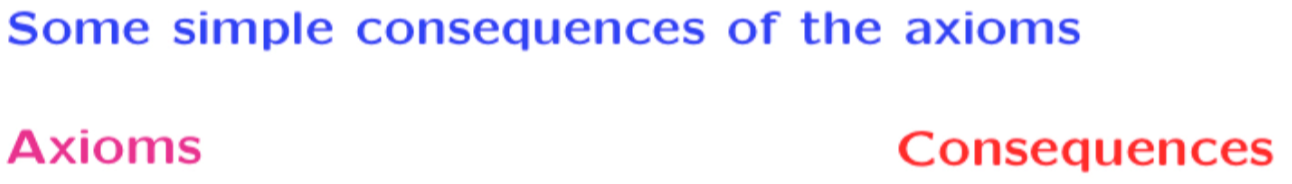
\includegraphics{AxiomConseqHead}
  \setfloatalignment{b}
\end{figure}

\begin{figure}
  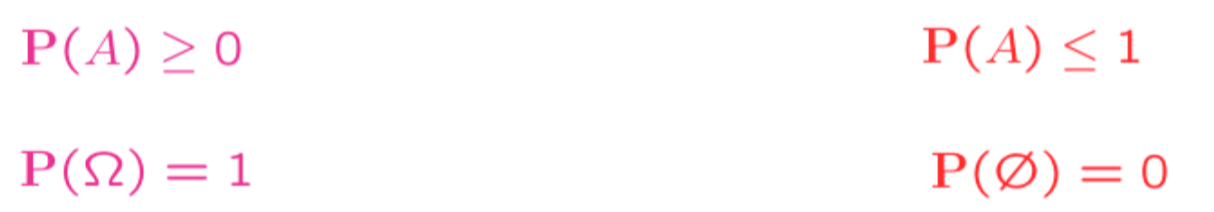
\includegraphics{AxiomConseq1}
\end{figure}

We also have another intuitive property. The probability that an event happens plus the probability that
the event does not happen exhaust all possibilities. And these two probabilities together should add to
1. For instance, if the probability of heads is 0.6, then the probability of tails should be 0.4.

Finally, we can generalize the additivity axiom, which was originally given for the case of two disjoint
events to the case where we're dealing with the union of several disjoint events. By disjoint here we
mean that the intersection of any two of these events is the empty set. We will prove this for the case of
three events and then the argument generalizes for the case where we're taking the union of k disjoint
events, where k is any finite number.

\begin{figure}
  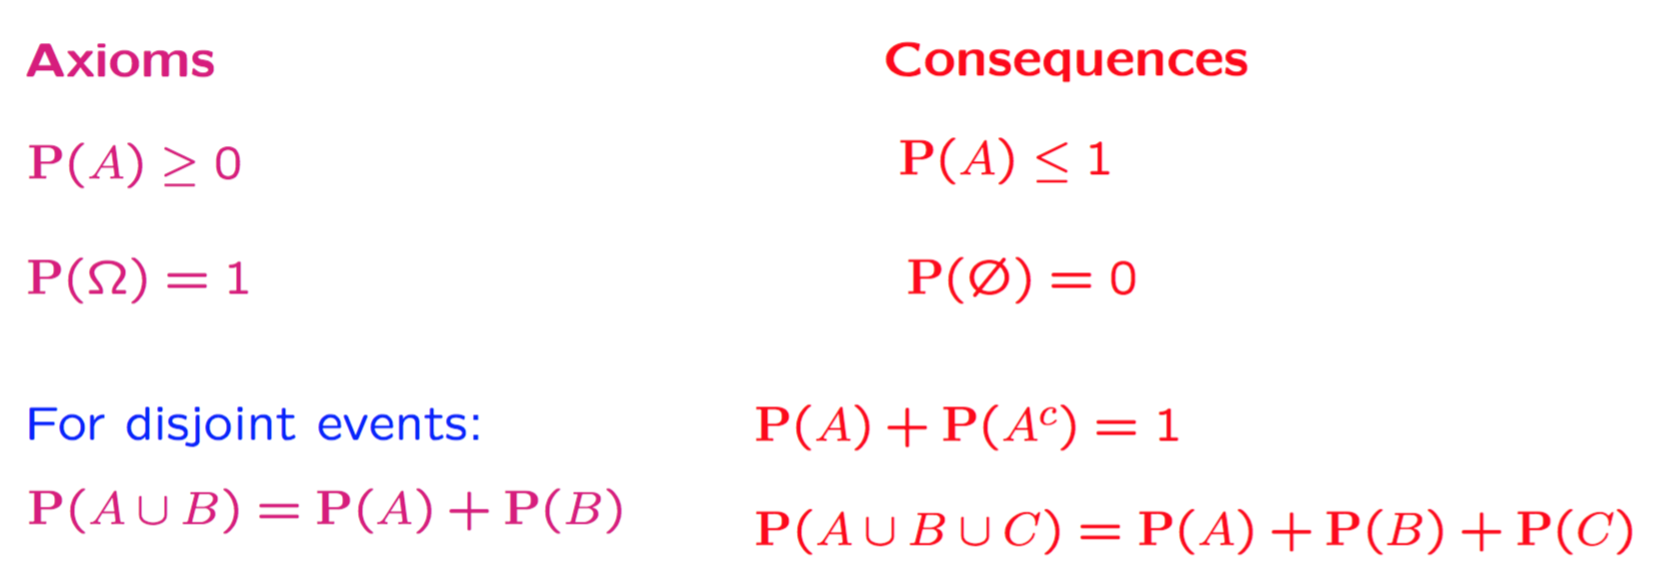
\includegraphics{AxiomConseq2}
\end{figure}

So the intuition of this result is the same as for the case of two events. But we will derive it formally and
we will also use it to come up with a way of calculating the probability of a finite set by simply adding the
probabilities of its individual elements.


All of these statements that we just presented are intuitive. And you do not to really need to be
convinced about their validity. \textit{Nevertheless}, it is instructive to see how these statements follow from the
axioms that we have put in place.

\newthought{So we will now present the arguments} based only on the three axioms that we have available. And in
order to be able to refer to these axioms, let us give them some names, call them axioms (a) (b), and (c):

\begin{marginfigure}
  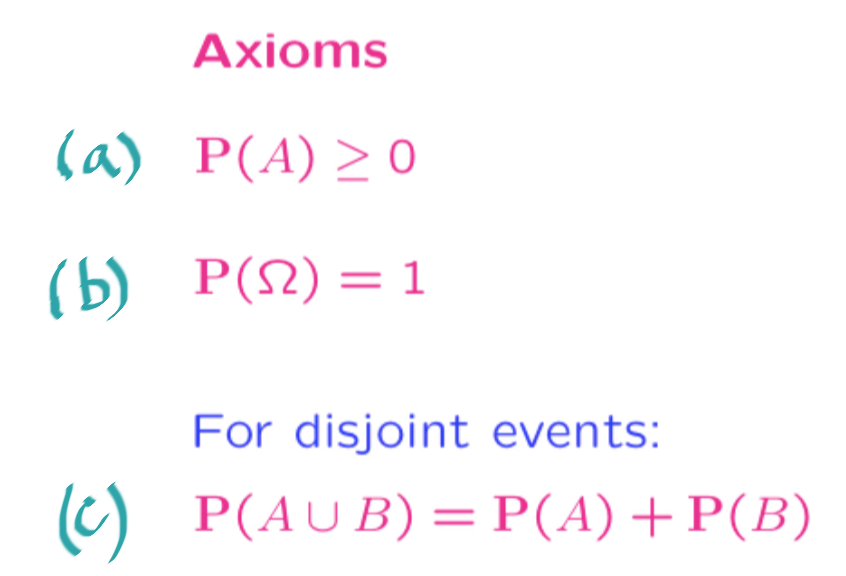
\includegraphics{Axioms}
  \setfloatalignment{b}
\end{marginfigure}



We start as follows. Let us look at the sample space and a subset of that sample space - call it A - and
consider the complement of that subset. The complement is the set of all elements that do not belong
to the set A. So a set together with its complement make up everything, which is the entire sample
space. On the other hand, if an element belongs to a set A, it does not belong to its complement. So the
intersection of a set with its complement is the empty set.
%\begin{figure}
\begin{marginfigure}
  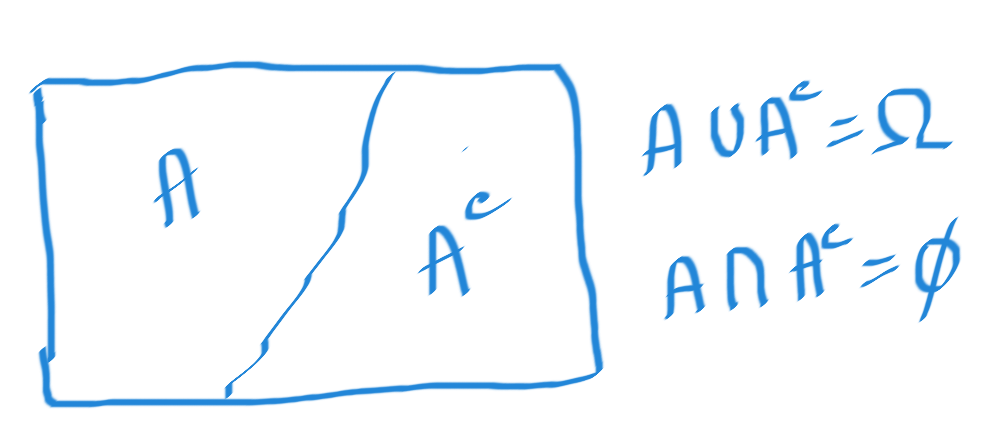
\includegraphics{AAcomplement}
  \caption{Complementary events make up the entire sample space $\Omega$.}
  \setfloatalignment{b}
%\end{figure}
\end{marginfigure}

\begin{marginfigure}
  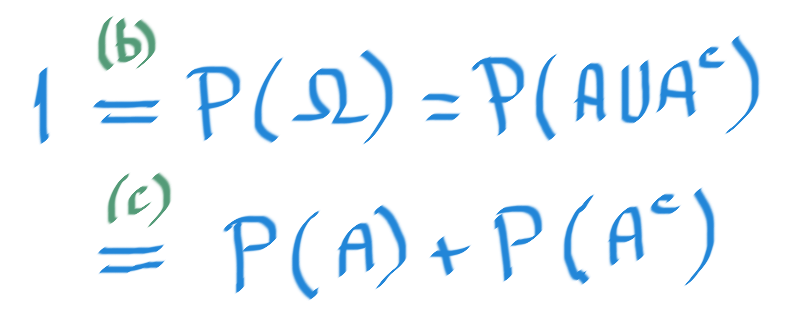
\includegraphics{DeriveComplement}
  \setfloatalignment{b}
%\end{figure}
\end{marginfigure}

Now we argue as follows. We have that the probability of the entire sample space is equal to 1. This is
true by our second axiom. Now the sample space, as we just discussed, can be written as the union of
an event and the complement of that event. This is just a set theoretic relation. Next, since a set and
its complement are disjoint, this means that we can apply the additivity axiom and write this probability
as the sum of the probability of event $A$ with the probability of the complement of $A$. This is one of the
relations that we had claimed and which we have now established.

\begin{marginfigure}
  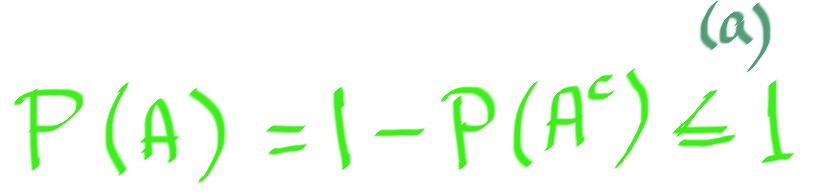
\includegraphics{ProbsLeq1}
  \caption{Thus we establish another property -- namely, that probabilities are always $\leq 1$.}
  \setfloatalignment{b}
\end{marginfigure}

Based on this relation, we can also write that the probability of an event A is equal to 1 minus the
probability of the complement of that event. And because, by the non-negativity axiom the quantity $P(A^c)$
is non-negative, 1 minus something non-negative is less than or equal to 1. Thus, by using the nonnegativity
axiom, we have established another property, namely that probabilities are always less
than or equal to 1.

Finally, let us note that 1 is the probability, always, of a set plus the probability of a complement of that
set. And let us use this property for the case where the set of interest is the entire sample space. Now,
the probability of the entire sample space is itself equal to 1. And what is the complement of the entire
sample space?

\begin{marginfigure}
  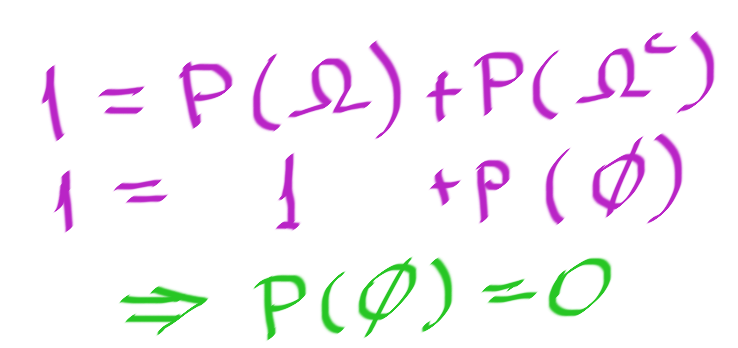
\includegraphics{ProbEmpty}
  \caption{Thus we establish yet another property -- namely, that the probability of the empty set is $0$.}
  \setfloatalignment{b}
\end{marginfigure}

The complement of the entire sample space consists of all elements that do not belong to the sample
space. But since the sample space is supposed to contain all possible elements, its complement is just
the empty set. And from this relation we get the implication that the probability of the empty set is equal
to 0. This establishes yet one more of the properties that we had just claimed a little earlier.

We finally come to the proof of the generalization of our additivity axiom from the case of two disjoint
events to the case of three disjoint events. We look at our sample space in Figure 4, and within that sample space
we have three events, three subsets. These subsets are disjoint in the sense that any two of those
subsets have no elements in common. We're interested in the probability of the union of $A$, $B$, and
$C$.

\begin{marginfigure}
  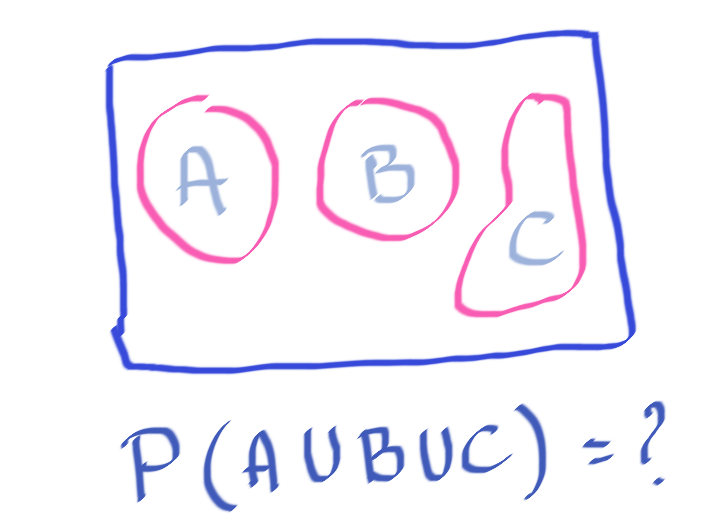
\includegraphics{UnionThree}
  \caption{Can we extend our additivity axiom (c) to three events? How about any finite number of disjoint events. Infinite number of disjoint events?}
  \setfloatalignment{b}
\end{marginfigure}


How do we make progress? We have an additivity axiom in our hands, which applies to the case of the
union of two disjoint sets. Here we have three of them. But we can do the following trick. We can think
of the union of $A$, $B$, and $C$ as consisting of the union of the set shaded in blue with that set shaded 
in green in Figure 5. Formally, what
we're doing is that we're expressing the union of these three sets as follows. We form one set by taking
the union of $A$ with $B$. And we have the other set $C$. And the overall union can be thought of as the
union of these two sets.

\begin{marginfigure}
  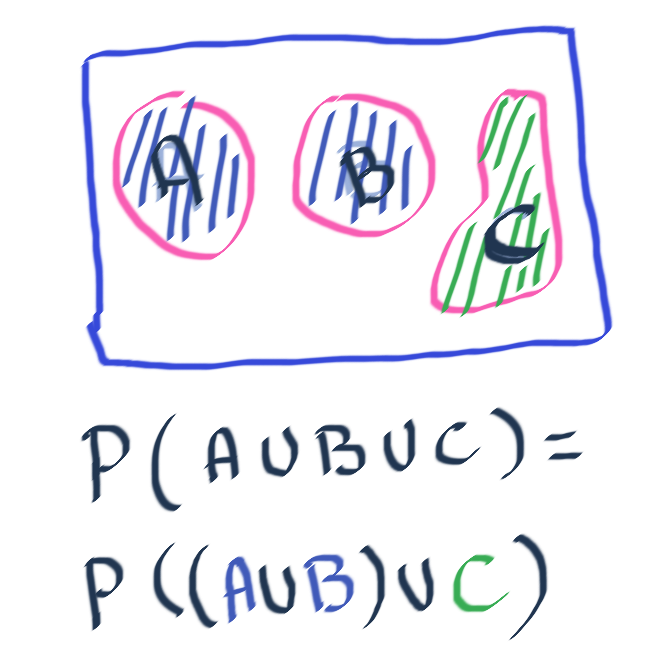
\includegraphics{UnionThree1}
  \caption{We can think of the union of events $A$ and $B$ as a single event $A \cup B$. We can then apply additivity  axiom to $A \cup B$ and $C$.}
  \setfloatalignment{b}
\end{marginfigure}


Now since the three sets are disjoint, this implies that the blue set is disjoint from the green set and so
we can use the additivity axiom here to write this probability as the probability of A union B plus the
probability of C. And now we can use the additivity axiom once more since the sets A and B are disjoint
to write the first term as probability of A plus probability of B. We carry over the last term and we have
the relation that we wanted to prove.

\begin{figure}
  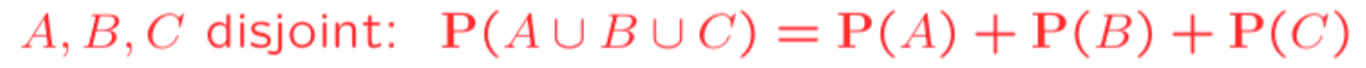
\includegraphics[width=10cm, height=5cm]{ThreeEventFormula}
  \setfloatalignment{b}
\end{figure}


\textit{This actually was the proof for the case of three events.} You should be able to follow this line of proof to write an
argument for the case of four events and so on. \textit{And you might want to continue by induction.} 
Eventually you should be able to prove that if the sets $A_1$ up to $A_k$ are disjoint then the probability of the
union of those sets is going to be equal to the sum of their individual probabilities. So this is the
generalization to the case where we're dealing with the union of finitely many disjoint events:

$$
\text{If } A_1, \ldots, A_K\text{ are disjoint } \implies P( A_1 \cup \ldots \cup A_K) = \sum_{i = 1}^K P(A_i)
$$



\newthought{\textit{Check Your Understanding: }}Let $A$, $B$, and $C$ be disjoint subsets of the sample space. For each one of the following statements, determine whether it is true or false. Note: "False" means "not guaranteed to be true."

\begin{align}
&P(A) + P(A^c) + P(B) = P(A \cup A^c \cup B) \\
&P(A) + P(B) \leq 1 \\
&P(A^c) + P(B) \leq 1 \\
&P(A \cup B \cup C) \geq P(A \cup B)
\end{align}

\begin{Answer} \ 
\begin{enumerate}
\item[a)] False. For a counterexample, let $A = \emptyset, B = \Omega,$ and $C = \emptyset$.
\item[b)] True. Sinse $A$ and $B$ are disjoint, we have $P(A) + P(B) = P(A \cup B) \leq 1.$
\item[c)] False. For a counterexample, let $A = \emptyset, B = \Omega,$ and $C = \emptyset$.
\item[d)] True. Since $A, B$, and $C$ are disjoint, we have 
\end{enumerate}
\end{Answer}



\pagebreak
%\vspace{0.5cm}
\section{More Consequenses of Axioms}\label{sec:axiom-consequences}

\newthought{Example 1.} We will now continue and derive some additional properties of probability laws which are, again,
consequences of the axioms that we have introduced. The first property is the following.

\begin{figure}[h]
  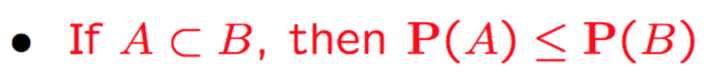
\includegraphics[width=6cm]{Conseq1}
  \setfloatalignment{b}
\end{figure}



\textit{We could argue why this is true as follows.} If we have two
sets and one set is smaller than the other, we have a picture similar to the one shown on the right. We have our sample
space. And we have some set, $A$.
We also have this set $B$, shown in figure 6, which is even bigger. So if B is a
set which is larger than A, then, naturally, the probability that the outcome falls inside B should be at
least as big as the probability that the outcome falls inside $A$.

\begin{marginfigure}
  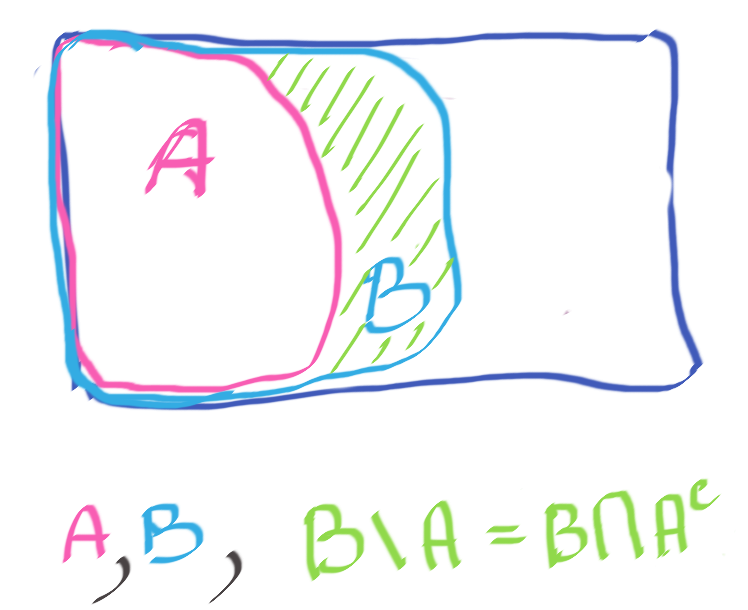
\includegraphics{AinB}
  \caption{Here $A$ is fully contained in $B$. The shaded part in green is that part of $B$ that does not contain any elements of $A$. This is denoted by $B \setminus A$. Another way to write this set: $B \cap A^c$.}
  \setfloatalignment{b}
\end{marginfigure}

How do we prove this formally? The set $B$ can be expressed as a union of two pieces. One piece is the
set $A$ itself. The second piece is whatever elements of $B$ there are that do not belong to $A$, which means that
they belong to the complement of $A$.

So we have expressed the set $B$ as the union of two pieces. One piece is $A$. The other piece is
outside $A$ - it is the one shaded in green in figure 6 and is that part of $B$ that does not include anything that belongs to $A$ also. Or, in set notation, $B \cap A^c$. This is sometimes also denoted as $B \setminus A$. Either way, these two pieces are disjoint. And so we can apply the additivity axiom, and write that the
probability of $B$ is equal to the probability of $A$ plus the probability of the other set.

\vspace{0.2cm}
\textit{Here is the exact same argument expressed more compactly using a mathematical notation.} First write set $B$ as follows: 
\begin{align*}
B = A \cup (B \cap A^c)
\end{align*}
The above line expresses $B$ as the union of two non-intersecting sets. So we can apply the additivity axiom, our axiom (c):
\begin{align*}
P(B )= P(A \cup (B \cap A^c)) = P(A) + P(B \cap A^c) \geq P(A)
\end{align*}

Since probabilities are non-negative, that is, since $P(B \cap A^c) \geq 0$, then indeed  we conclude that the probability of $A$ is less than or equal to the probability of $B.$ $\Box$


\newthought{Example 2.} The next property we will show allows us to write the probability of the union of two
sets for the case now, where the two sets are not necessarily disjoint. 

\begin{figure}
  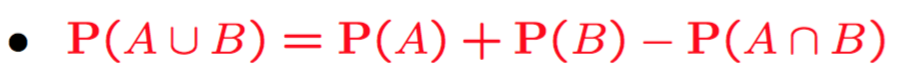
\includegraphics[width=7cm]{Conseq2}
  \setfloatalignment{b}
\end{figure}

So the picture is as follows. We
have our two sets, A and B. These sets are not necessarily disjoint. And we want to say something
about the probability of the union of A and B.

\begin{marginfigure}
  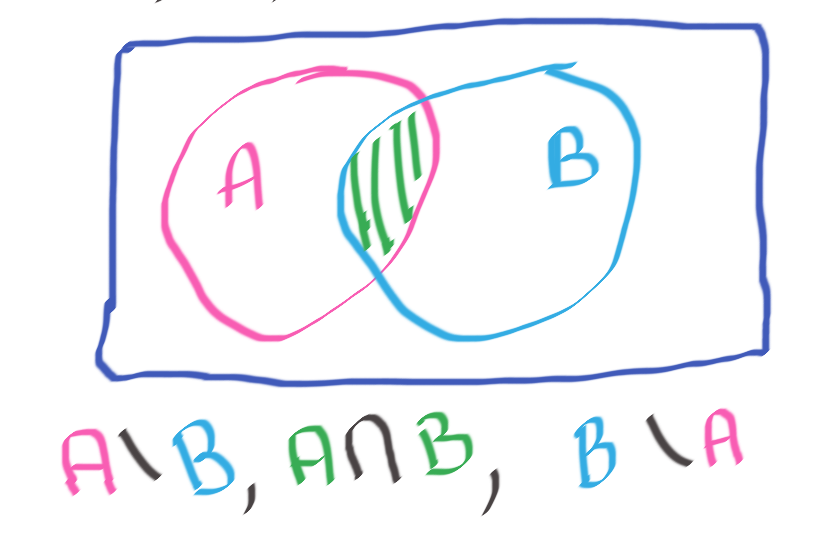
\includegraphics{AintersectsB}
  \caption{Here $A$ and $B$ \textit{do} intersect. But the union of $A$ and $B$ can be represented as the union of the three non-intersecting sets $A \setminus B, A \cap B$ and $B \setminus A$.}
  \setfloatalignment{b}
\end{marginfigure}


Can you prove that $P(A \cup B) = P(A) + P(B) - P(A \cap B)$? Use the picture shown on the right and try to use either the mathematical notation or argue it verbally, as we did in example 1.

\vspace{0.2cm}
\textit{Here is a hint if you get stuck:} $A \cup B$ can be expressed as the union of non intersecting sets $A\cup B^c, A \cap B$ and $B \cup A^c$. Denote the probabilities of these sets by $a, b, c$, respectively. What is then $P(A \cup B)$ in terms if $a, b$ and $c$? It is $a + b +c$. On the other hand, can you express $P(A) + P(B) - P(A \cap B)$ in terms of $a, b, c$ as well? If the anwer to this is also $a + b +c$, then you've got your proof. \textit{Further hint:}  note that $P(A) = a + b$ and $P(B) = b + c$.  $\Box$

\newthought{Example 3.} Here's yet another consequequence of the three axioms:

\begin{figure}
  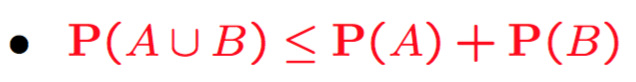
\includegraphics[width=5.5cm]{Conseq3}
  \setfloatalignment{b}
\end{figure}

Can you see why this is true? This should follow right from the previous example. Recall that the probabilities are non-negative and thus, looking at what we proved in example 2, since $P(A \cap B) \geq 0$, it must follow that $P(A \cup B) \geq P(A) + P(B)$. 

In fact, this inequality even has a name. It's called the \textit{union bound inequality}. $\Box$


\newthought{\textit{Check Your Understanding: }}Let $A$, $B$, and $C$ be subsets of the sample space, not necessarily disjoint. For each one of the following statements, determine whether it is true or false. Note: "False" means "not guaranteed to be true."

\setcounter{equation}{0}
\begin{align}
&P(A \cup B \cup C)  = P(A) + P(A^c \cap B) + P (A^c \cap B^c \cap C) \\
&P((A \cap B) \cup (C \cap A^c)) \leq P(A \cup B \cup C) \\
&P(A \cup B \cup C) = P(A \cap C^c) + P(C) + P(B \cap A^c \cap C^c)
\end{align}




\pagebreak
\section{We now move from the abstract to the concrete :)}\label{sec:model-building}

\begin{marginfigure}
  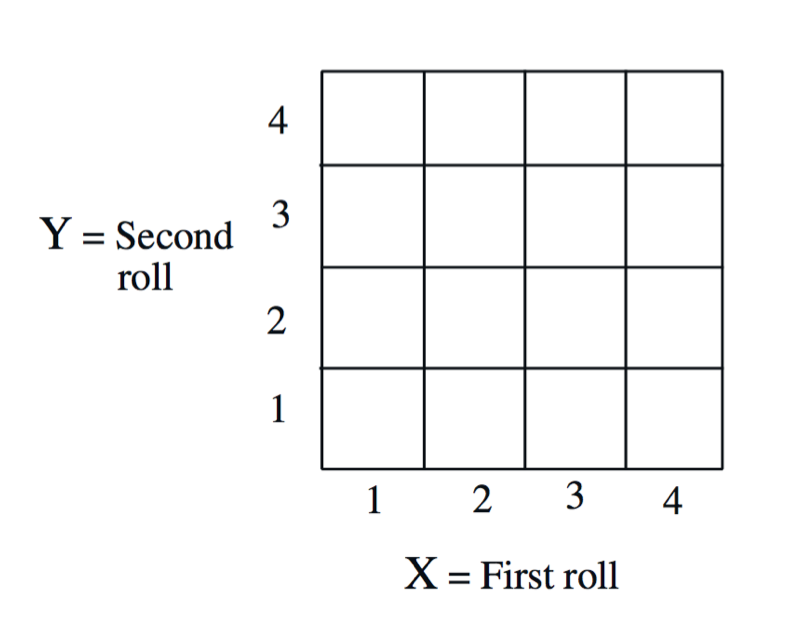
\includegraphics{TetraDie}
  \caption{The tetrahedral die we saw earlier. Let's now \textit{make an assumption}nthat the 16 possible outcomes are all
equally likely.}
  \setfloatalignment{b}
\end{marginfigure}

Recall the example that we discussed earlier where
we have two rolls of a tetrahedral die. So there are 16 possible outcomes shown in figure 8. To
continue, we need to specify a probability law, some kind of probability assignment.

To keep things simple, we're going to make the assumption that the 16 possible outcomes are all
equally likely. And each outcome has a probability of 1 over 16. Given this assumption, we will now
proceed to calculate certain probabilities.

\begin{marginfigure}
  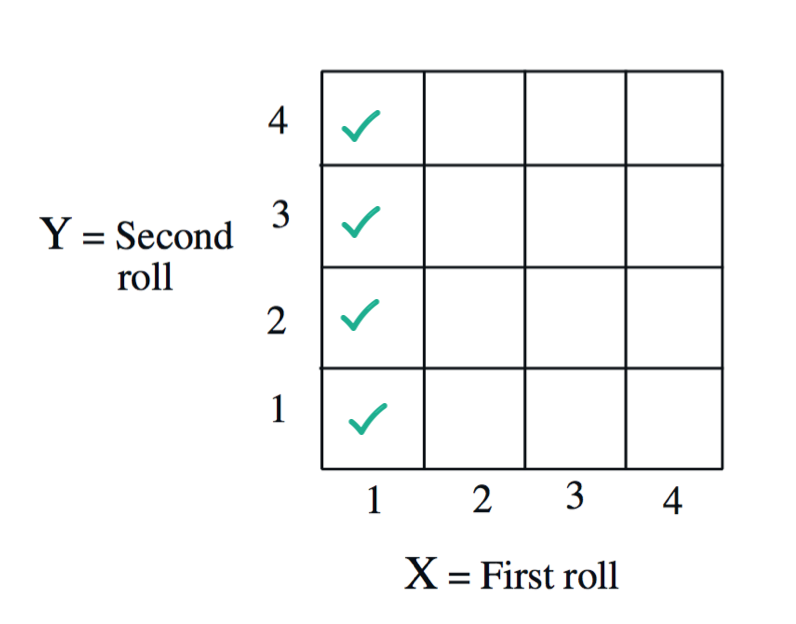
\includegraphics{CheckMarkedDie}
  \caption{The checkmarked boxes correspond to the two rolls of the die that resulted in the first roll showing face 1.  The pribability of this event works out to be $\frac{1}{4}.$}
  \setfloatalignment{b}
\end{marginfigure}


Let us look first at the probability that $X$, which stands for "the result of the first roll", is equal to $1$. The way to
calculate this probability is to identify what exactly that event is in our picture of the sample space, and
then calculate. The event that $X = 1$ can happen in four different ways that correspond to these
four particular outcomes.

Each one of these outcomes has a probability of 1 over 16. The probability of this event is the sum of
the probabilities of the outcomes that it contains. So it is $4 \times \frac{1} {16} = \frac{1} {4}.$

\vspace{3.4cm}
Let now $Z$ stand for the smaller of the two numbers that came up in our two rolls. So for example, if $X$ is
2 and $Y$ is equal to 3, then $Z$ is equal to 2, which is the smaller of the two. 

Let us try to calculate the
probability that the smaller of the two outcomes is equal to 4.

\begin{marginfigure}
  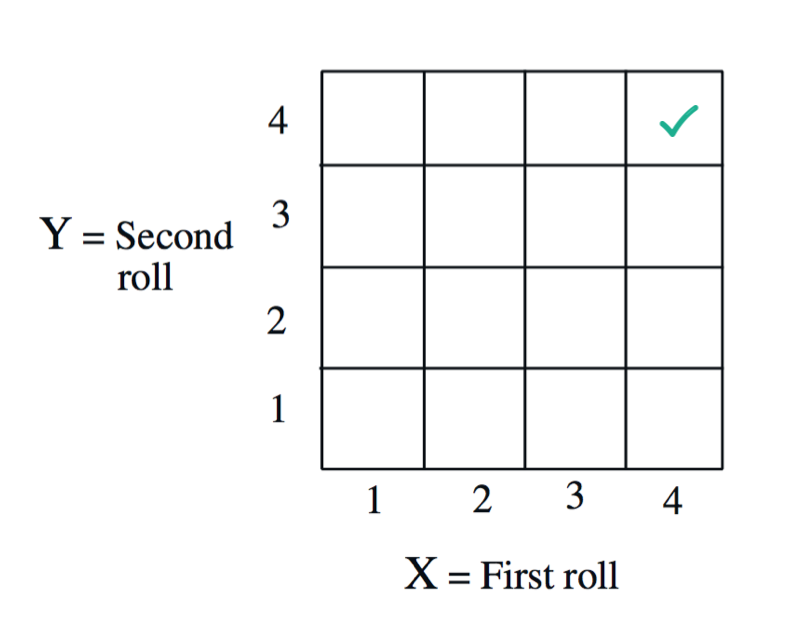
\includegraphics{CheckMarkedDie2}
  \caption{The checkmark now corresponds to the event that the smaller of the two faces of the die came up equal to 4. There is only one such outcome -- namely, when both rolls result in a 4. Its probability is then $\frac{1}{16}.$ }
  \setfloatalignment{b}
\end{marginfigure}

Now, for the smaller of the two outcomes to be equal to 4, we must have that both $X$ and $Y$ are equal to
4. So this top rightmost square in figure 10 is the only way that this particular event can happen. Since there's only one
outcome that makes the event happen, the probability of this event is the probability of that outcome
and is equal to $\frac{1}{16}$.

%\vspace{2cm}
\pagebreak
For another example, let's calculate the probability that the minimum is equal to 2. What does it mean
that the minimum is equal to 2? It means that one of the dice resulted in a 2, and the other die resulted
in a number that's 2 or larger. So we could have both equal to 2. We could have $X$ equal to 2, but $Y$
larger. Or we could have $Y$ equal to 2 and $X$ something larger.

\begin{marginfigure}
  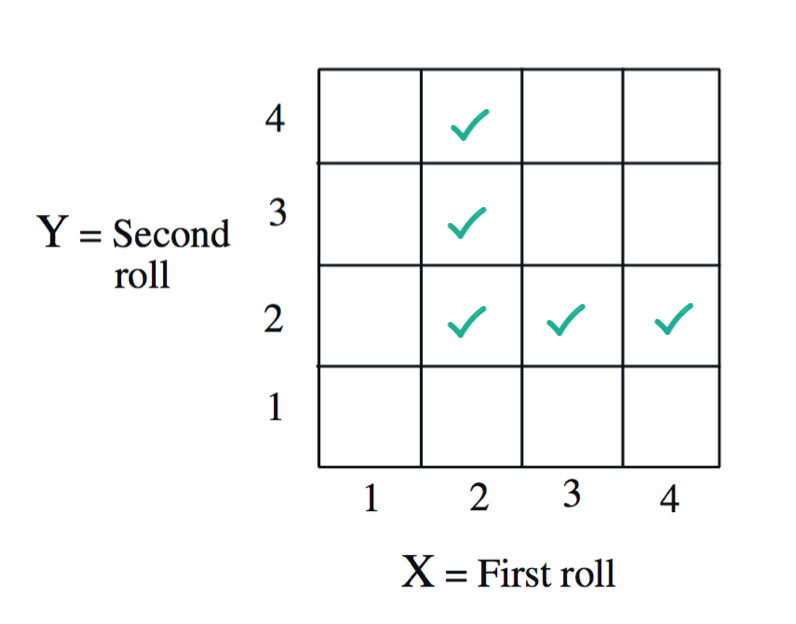
\includegraphics{CheckMarkedDie3}
  \caption{The checkmark now corresponds to the event that the smaller of the two faces of the die came up equal to 2. There are 5 such outcomes -- namely, the ones checkmarked in this figure. The probability of this event is $\frac{5}{16}.$ }
  \setfloatalignment{b}
\end{marginfigure}

The checkmarked boxes on this figure to the right correspond to all outcomes for which the minimum of the two rolls is
equal to 2. There's a total of five such outcomes. Each one of them has probably 1 over 16. And we
have discussed that for finite sets, the probability of a finite set is the sum of the probabilities of the
elements of that set. So we have five elements here, each one with probability 1 over 16. And the
answer to this problem is then $\frac{5}{16}$.


\vspace{0.3cm}
\begin{marginfigure}
  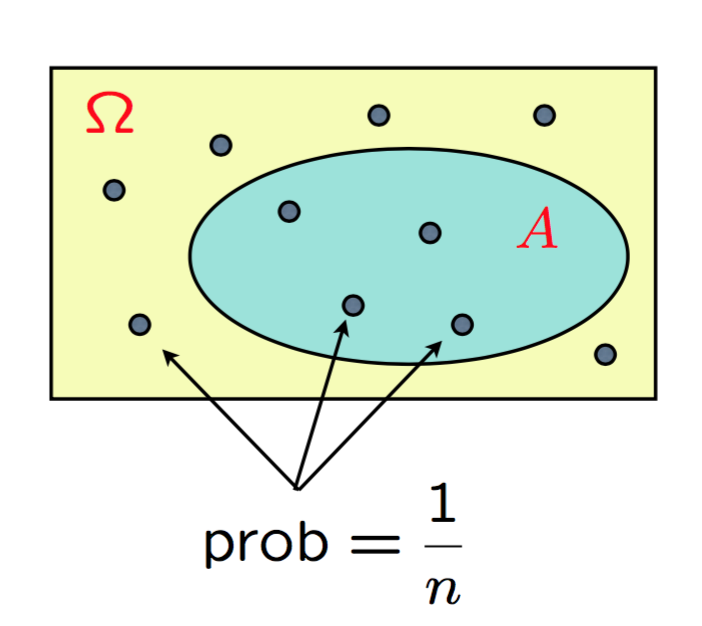
\includegraphics{DiscreteUniform}
  \caption{\textbf{Discrete Uniform Law.} Here $\Omega$ has finite number of elements, $n$, and each is equally likely to occur, 
  that is, each has probability of $\frac{1} {n}$ of occuring. Set $A$ contains $k$ elements. Then $P(A) = k \cdot \frac{1} {n} = \frac{k} {n} $ .}
  \setfloatalignment{b}
\end{marginfigure}

\newthought{This particular example} that we just saw is a special case of what is called a discrete uniform law. In a
discrete uniform law, we have a sample space which is finite. And it has n elements, and we assume
that these n elements \textit{are equally likely}. Now since the probability of the entire
sample space $\Omega$ is equal to 1, this means that each one of these elements must have probability $1/n$. That's the only way that the sum of the probabilities of the different outcomes would be equal to 1 as
required by the normalization axiom.


Consider now some subset of the sample space, an event $A$ that, exactly $k$ elements. What is the
probability of the set $A$? It's the sum of the probabilities of its elements. There are k elements. And each
one of them has a probability of 1 over n. And this way we can find the probability of the set $A$. It is $k \times \frac{1}{n}$.

So when we have a discrete uniform probability law, we can calculate probabilities by simply counting
the number of elements of omega, which is $n$, finding the number $n$, and counting the number of
elements of the set $A$. \textit{That's the reason why counting will turn out to be an important skill. And there will
be a whole lecture devoted to this particular topic.}

\newthought{\textit{Check Your Understanding: }}Consider the same model of two rolls of a tetrahedral die, with all 16 outcomes equally likely. Find the probability of the following events:
\begin{enumerate}
\item The value in the first roll is strictly larger than the value in the second roll.
\item The sum of the values obtained in the two rolls is an even number.
\end{enumerate}





\subsection{}\label{sec:outcomes}






\vspace{0.5cm}



\section{Probability calculation, a continuous example}\label{sec:continuous-example}

We will now go through a probability calculation for the case where we have a continuous sample
space. We revisit our earlier example in which we were throwing a dart into a square target, the square
target being the unit square. And we were guaranteed that our dart would fall somewhere inside this
set. So our sample space is the unit square itself.

\begin{marginfigure}
  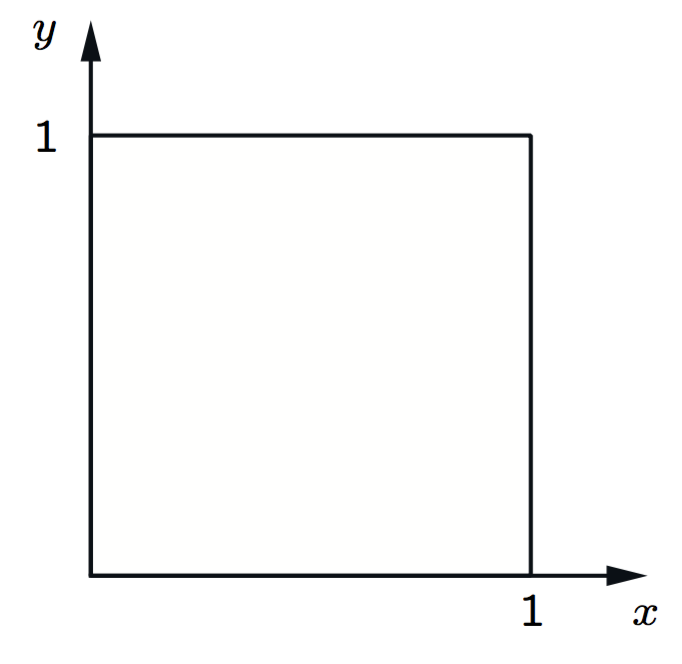
\includegraphics{ContSampleSpace}
  \caption{An example of a continuous sample space: $\Omega$ consists of all $(x, y)$ such that $0 \leq x, y \leq 1$.}
  \setfloatalignment{b}
\end{marginfigure}


We have a description of the sample space, but we also need to
specify a probability law. The choice of a probability law could be arbitrary. It's up to us to choose how to model a
certain situation. And to keep things simple, we're going to assume that our probability law is a uniform
one, which means that the probability of any particular subset of the sample space is going to be the
area of that subset.

\begin{figure}
  
\includegraphics[width=8cm]{UniformLaw}
  \setfloatalignment{b}
\end{figure}


So if we have some subset lying somewhere in the unit square and we ask what is the probability that we fall into
that subset? The probability is exactly the area of that particular subset. Once more, this is an arbitrary
choice of a probability law. There's nothing in our assumptions so far that would force us to make this
particular choice. And we just use it for the purposes of this example.


So now let us calculate some probabilities. Let us look at this event. This is the event that the sum of
the two numbers that we get in our experiment is less than or equal to 1/2: 

$$
P\left(  \{(x, y) \mid x + y \leq 1/2   \}   \right) = \ ?
$$

It is always useful to work in
terms of a picture and to depict that event in a picture of the sample space. So in terms of that sample
space, the points that make this event to be true are just a triangle that lies below the red line shown in
this picture, that's x plus y equals 1/2. Below that line are the outcomes that make this
event happen.

\begin{marginfigure}
  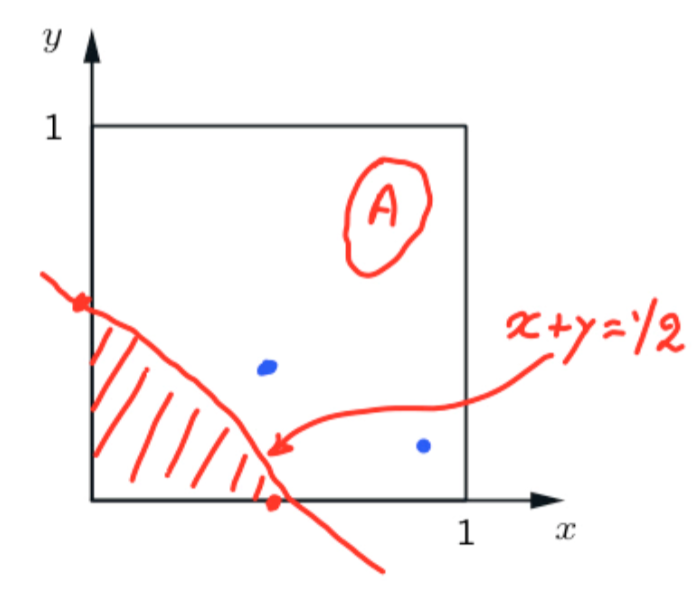
\includegraphics{ContSampleSpace1}
  \caption{We are interested in $(x, y)$ such that $x + y \leq 1/2$.}
  \setfloatalignment{b}
\end{marginfigure}

So we're trying to find the probability of the event shaded in red in Figure 14. We have assumed that probability is equal to
area. Therefore, the probability we're trying to calculate is the area of a triangle. And the area of a
triangle is 1/2 times the base of the triangle, which is 1/2 in our case, times the height of the triangle,
which is again 1/2 in our case. And the end result is 1/8:

$$
P\left(  \{(x, y) \mid x + y \leq 1/2   \}   \right) = \frac{1}{2} \cdot \frac{1}{2} \cdot \frac{1}{2} = \frac{1}{8} 
$$

\vspace{0.7cm}
Let us now calculate another probability - let's find the probability of an event that consists of only a single element. We
take the point 0.5, 0.3, which sits somewhere in the square. The event of interest is a set, but that set consists of
a single point. So we're asking for the probability that our dart falls exactly on top of that point.

What is it? Well, it is the area of a set that consists of a single point. What is the area of a single point?
It is 0. And similarly for any other single point inside that sample space that we might have considered,
the answer is going to be 0.

\vspace{0.7cm}
Let us now abstract from this example, as well as the previous one, and note the following. Probability
calculations involve a sequence of four steps. Starting with a word description of a problem, of a
probabilistic experiment, we first write down the sample space. 

\begin{marginfigure}
  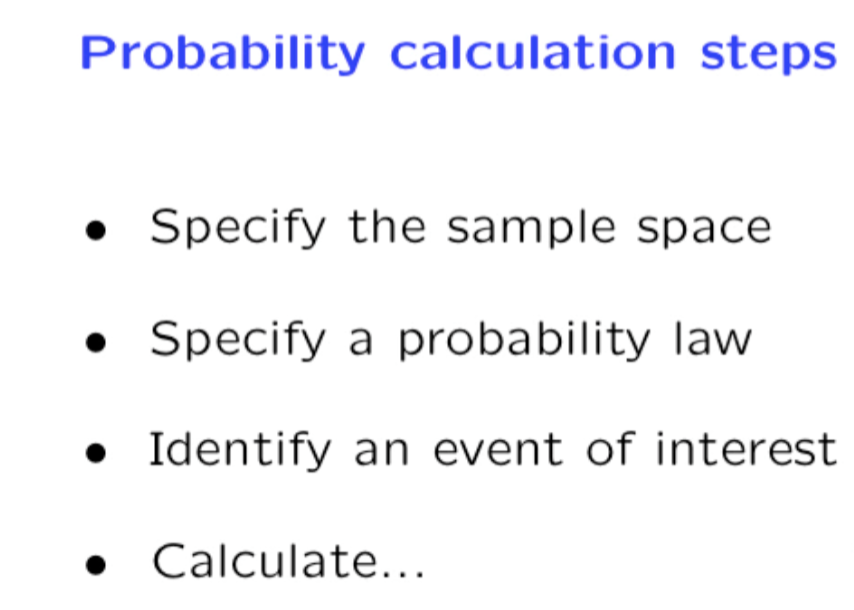
\includegraphics{StepsOfProbCalc}
  \setfloatalignment{b}
\end{marginfigure}

Then we specify a probability law. Let me emphasize again here that this step has some arbitrariness in it. You can choose any probability
law you like, although for your results to be useful it would be good if your probability law captures the
real-world phenomenon you're trying to model.

 Next, typically you're interested in calculating the probability
of some event. That event may be described in some loose manner, so you need to describe it
mathematically. And if possible, it's always good to describe it in terms of a picture. Pictures are
immensely useful when going through this process.

And finally, the last step is to go ahead and calculate the probability of the event of interest. Now, a
probability law in principle specifies the probability of every event, and there's nothing else to do. But
quite often the probability law will be given in some implicit manner, for example, by specifying the
probabilities of only some of the events. In that case, you may have to do some additional work to find
the probability of the particular event that you care about.

This last step sometimes will be easy. Sometimes it may be complicated. But in either case, by following
this four-step procedure and by being systematic you will always be able to come up with a single
correct answer.

\pagebreak
\section{Probability calculation, discrete but infinite sample space}\label{sec:continuous-example}

We have seen so far an example of a probability law on a discrete and finite sample space as well as
an example with an infinite and continuous sample space. Let us now look at an example involving a
discrete but infinite sample space.

We carry out an experiment whose outcome is an arbitrary positive integer. As an example of such an
experiment, suppose that we keep tossing a coin and the outcome is the number of tosses until we
observe heads for the first time. The first heads might appear in the first toss or the second or the third,
and so on. So in this example, any positive integer is possible. And so our sample space is infinite.


\begin{marginfigure}
  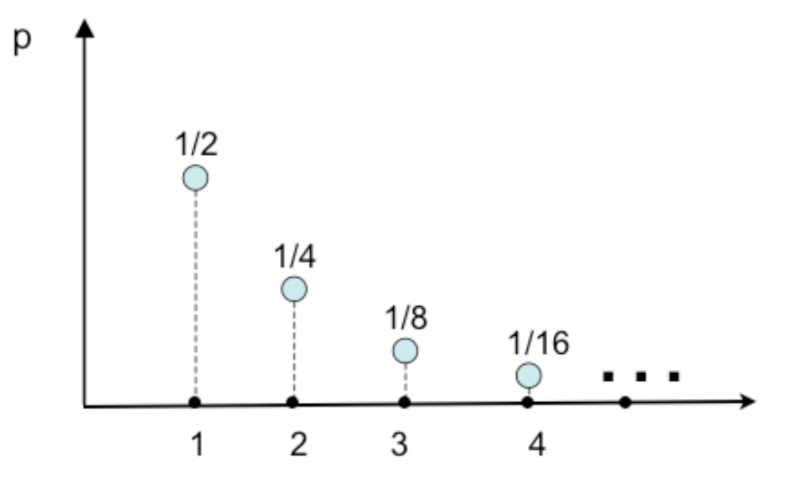
\includegraphics{InfiniteSampleSpace}
  \caption{An example of a discrete but infinite sample space.}
  \setfloatalignment{b}
\end{marginfigure}

Let us now specify a probability law. A probability law should determine the probability of every event, of
every subset of the sample space. That is, the probability of every set of positive integers. But instead I
will just tell you the probability of events that contain a single element. I'm going to tell you that there is
probability $1/2^n$ that the outcome is equal to $n$:

$$
P(n) = \frac{1}{2^n}
$$


Is this information good
enough to determine the probability of \textit{any} subset?

Before we look into that question, let us first do a quick sanity check to see whether these numbers that
we are given look like legitimate probabilities. Do they add to 1? Let's do a quick check. So the sum
over all the possible values of n of the probabilities that we're given, which is an infinite sum starting
from 1, all the way up to infinity, of $1/2^n$, is equal to the following:

$$
\sum_{n=1}^{\infty} \frac{1}{2^n} = \frac{1}{2} \sum_{n=0}^{\infty} \frac{1}{2^n} 
$$

And now on the right side we have a usual infinite geometric series and we have a formula for this:
$\sum_{n=0}^{\infty} \frac{1}{2^n}  = \frac{1}{1 - 1/2}$ . Thus
\begin{align*}
\sum_{n=1}^{\infty} \frac{1}{2^n} &= \frac{1}{2} \cdot \frac{1}{1 - 1/2}\\
&= \frac{1}{2} \cdot 2\\
&= 1
\end{align*}

So indeed, \textit{it appears }that we have the basic elements of what
it would take to have a legitimate probability law.


\vspace{0.4cm}
But now let us look into how we might calculate the probability of some general event. For example, the
probability that the outcome is even. We proceed as follows. The probability that the outcome is even 
is the probability of an infinite set that consists of all the even integers. We can write this set as the
union of lots of little sets that contain a single element each. So it's the set containing the number 2, the
set containing the number 4, the set containing the number 6, and so on:


\begin{align*}
P( \text{outcome is even}) &= P(\{ 2, 4, 6, \ldots, \})\\
&= P(\{ 2\} \cup \{ 4\} \cup \{ 6\} \cup \ldots) \\
&= P(\{ 2\}) + P(\{ 4\}) + P(\{ 6\}) \ldots
\end{align*}

The last equality follows because we notice that we're talking about the probability of a union of sets and these sets are
disjoint because they contain different elements. So we can use an additivity property and say that this
is the probability of obtaining a 2, plus the probability of obtaining a 4, plus the probability of obtaining a
6 and so on.

If you're curious about doing this calculation and actually obtaining a numerical answer, you would
proceed as follows. You notice that the last expression above equals to:

\begin{align*}
\frac{1}{2^2} + \frac{1}{2^4} + \frac{1}{2^6}  \ldots &=  \frac{1}{4} \cdot (1 + \frac{1}{4} + \frac{1}{4^2}  \ldots )\\
  &=  \frac{1}{4} \cdot  \frac{1}{ 1 -  1/4} \\
 &= \frac{1}{3} 
\end{align*}

Thus the probability that the outcome of this experiment is an even number is 1/3. Does this result sound intuitive to you?

Leaving the details of the calculation aside, the more important question I want to address is the
following. Is this calculation correct? We seem to have used an additivity property at this point. But the
additivity properties that we have in our hands at this point only talk about disjoint unions of finitely
many subsets.

Our initial axiom talked about a disjoint union of two subsets and then later on we established a similar
property for a disjoint union of finitely many subsets. But here we're talking about the union of infinitely
many subsets. So this step of taking an infinite union is not really allowed by what we have in our hands. 

On the other hand,
we would like our theory to allow this kind of calculation.

The way out of this dilemma is to introduce an additional axiom that will indeed allow this kind of
calculation. The axiom that we introduce is the following. If we have an infinite sequence of disjoint
events, as for example in this picture. We have our sample space. We have a first event, $A_1$. We have a
second event, $A_2$. The third event, $A_3$. And so we keep continuing and we have an infinite \textit{sequence of
such events}. Then the probability of the union of these events, of these infinitely many events, is the
sum of their individual probabilities.

\begin{figure}
  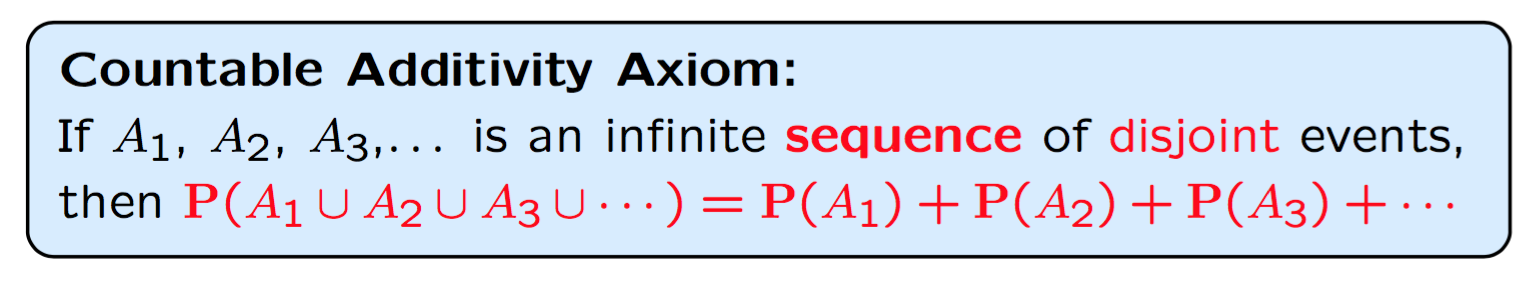
\includegraphics{CountableAdditivityAxiom}
  \setfloatalignment{b}
\end{figure}


The key word here is the word \textbf{sequence}. Namely, these events, these sets that we're dealing with, can
be arranged so that we can talk about the first event, $A_1$, the second event, $A_2$, the third one, $A_3$, and
so on.

\begin{marginfigure}
  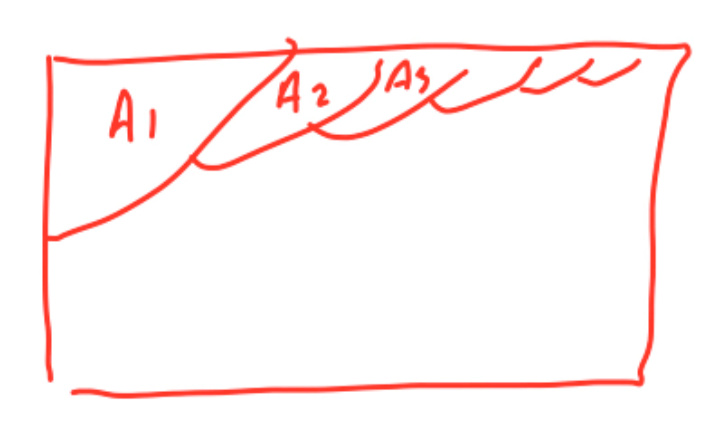
\includegraphics{EventSequence}
  \caption{An infinite sequence of events.}
  \setfloatalignment{b}
\end{marginfigure}


To appreciate the issue that arises here and to see why the word sequence is so important, let us
consider the following calculation. Our sample space is the unit square. And we consider a model where
the probability of a set is its area, as in the examples that we considered earlier. Let us now look at the
probability of the overall sample space. Our sample space is the unit square and the unit square can be
thought of as the union of various sets that consist of single points. So it's the union of subsets with one
element each. And it's a union taken over all the points in the unit square.

\begin{marginfigure}
  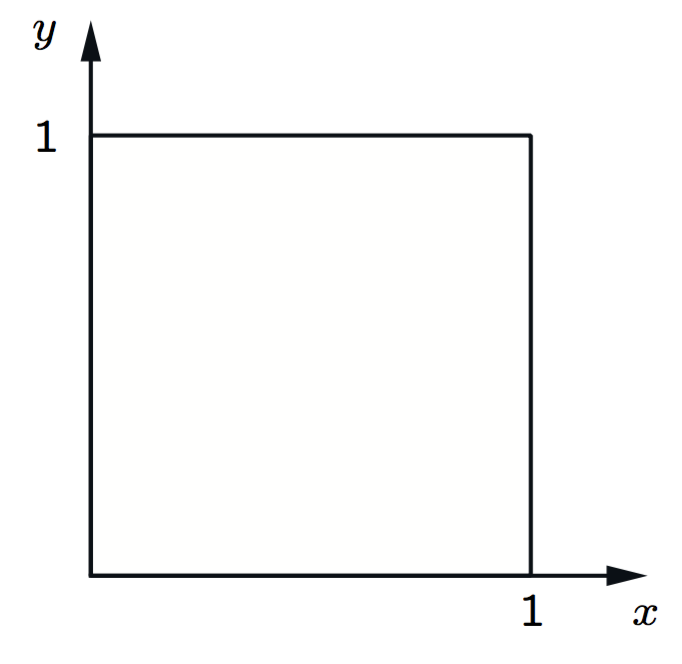
\includegraphics{ContSampleSpace}
  \caption{The unit square again. Each point has zero probability in our model. All points make up the entire square, which has probability 1. There is an infinite number of such points. Can the sum of these infinitely many zeros add up to one?}
  \setfloatalignment{b}
\end{marginfigure}


Then we think about additivity. We observe that these subsets are disjoint. If we're considering different
points, then we get disjoint single element sets. And then an additivity property would tells us that the
probability of these union is the sum of the probabilities of the different single element subsets.

Now, as we discussed before, single element subsets have 0 probability. So we have a sum of lots of 0s
and the sum of 0s should be equal to 0. On the other hand, by the probability axioms, the probability of
the entire sample space should be equal to 1. 

\begin{align*}
1 = P(\Omega) &=  P ( \cup \{ x, y\} ) \\
&=  \sum P(\{ x, y\} ) = \sum 0 = 0
\end{align*}

And so we have established that 1 is equal to 0. 

\vspace{0.3cm}
This
looks like a paradox. Is it? 

\vspace{0.3cm}
The catch is that there is nothing in the axioms we have introduced so far or
the properties we have established that would justify the step that says
$P ( \cup \{ x, y\} ) = \sum P(\{ x, y\} ) $ in these calculations. This is the step that's questionable!


You might argue that the unit square is the union of disjoint single element sets, which is the case that
we have in additivity axioms. But the additivity axiom only applies when we have a sequence of events.
And this is not what we have here. This is not a union of a sequence of single element sets. In fact,
there is no way that the elements of the unit square can be arranged in a sequence. The unit square is
said to be an uncountable set.

\begin{figure}
  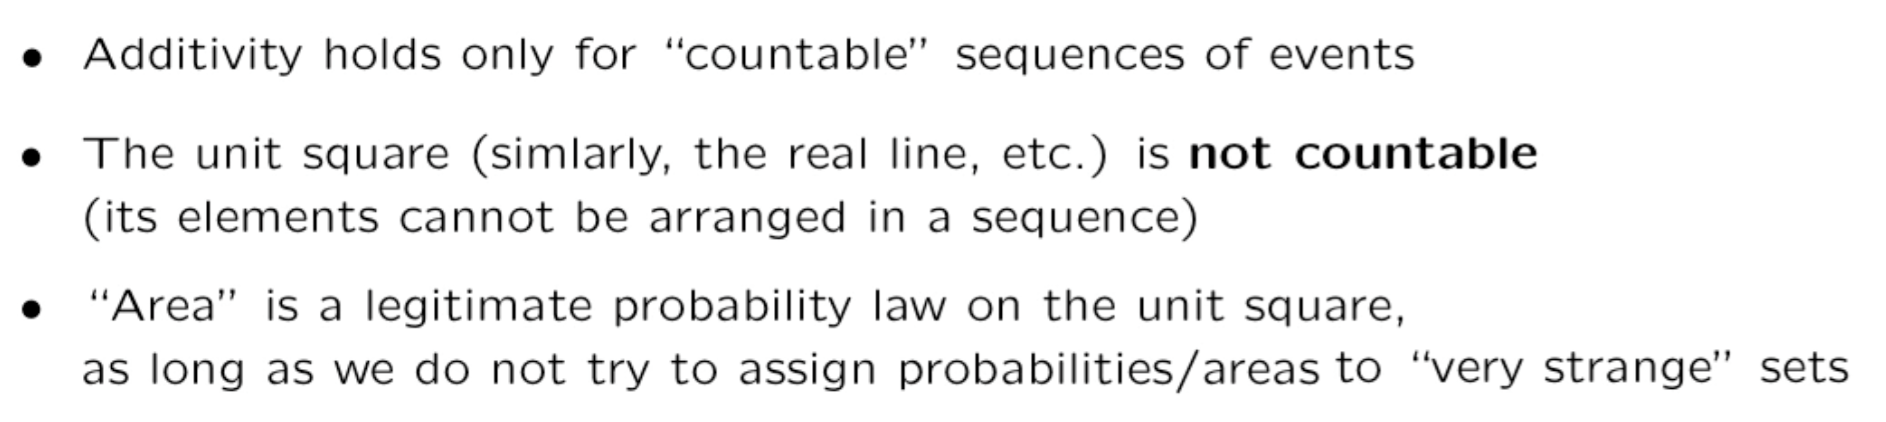
\includegraphics{NoCountable}
  \setfloatalignment{b}
\end{figure}


This is a deep and fundamental mathematical fact. What it essentially says is that there are two kinds of
infinite sets. Discrete ones, or, in formal terminology, countable. These are sets whose elements can be
arranged in a sequence, like the integers. 

And then there are uncountable sets, such as the unit square or the
real line, whose elements cannot be arranged in a sequence. If you're curious, you can find the proof of
this important fact in supplementary materials (ask me).

\vspace{0.3cm}
After all these discussions, you may now have legitimate suspicions about the models we have been
looking at. Is area a legitimate probability law? Does it even satisfy countable additivity? This question
takes us into deep waters and has to do with a deep subfield of mathematics called Measure Theory.

Fortunately, it turns out that all is well. Area is a legitimate probability law. It does indeed satisfy the
countable additivity axiom as long as we only deal with nice subsets of the unit square. Fortunately, the
subsets that arise in whatever we do in this course will be "nice". Subsets that are not nice are quite
pathological and we will not encounter them.

At this stage we are not in a position to say anything more that would be meaningful about these issues
because they're quite complicated and mathematically deep. We can only say that there are some
serious mathematical subtleties. But fortunately, they can all be overcome in a rigorous manner. And for
the rest of this class, you can just forget about these subtle issues.


\end{document}


\newthought{\textit{Check Your Understanding: }} Let $A$ and $B$ be events, with $P(A)=0.6$ and $P(B)=0.7$. Can these two events be disjoint?





